\section{Results and Analysis}

\subsection{The Arrow}
	\label{sec:arrow}
We chose to use a paper airplane model called ``The Arrow" to conduct the experiments. See Figure~\ref{fig:arrow} for a picture of The Arrow. We chose this model because it is easy to construct and rigid in structure. Due to its relatively small wing aspect ratio, The Arrow experiences little flapping motion; as a result, its flight better resembles what is assumed in theory. We constructed three The Arrow paper airplanes in order to reduce any model-specific measurement error. All results came from an average of these three models. See Figure~\ref{fig:arrowdimension} for the weight and dimensions of these three airplanes. 

\begin{figure}[hl]
  \centering
    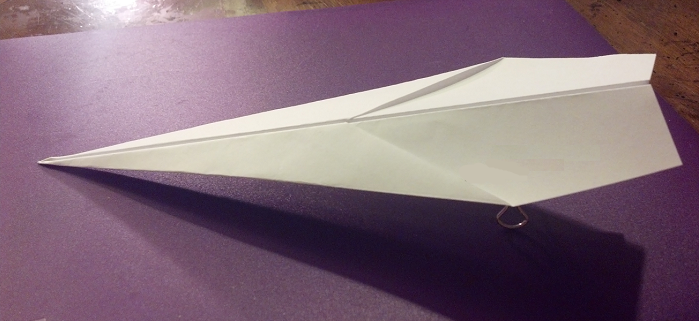
\includegraphics[scale=0.6]{figures/arrow.png}
    \caption{A picture of The Arrow. It is one of the most common paper airplane models. It has a long flight range and is easy to construct.}
  \label{fig:arrow}
\end{figure}

\begin{figure}[hl]
  \centering
    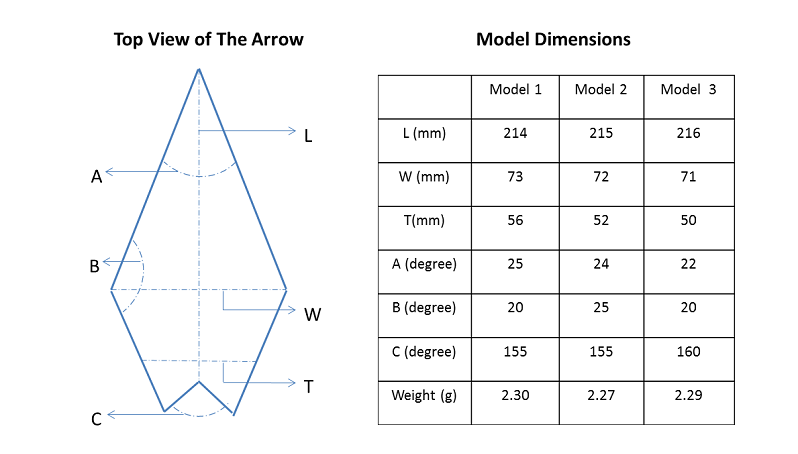
\includegraphics[scale=0.6]{figures/arrowdimension.png}
    \caption{Weight and dimension of the three paper airplanes.}
  \label{fig:arrowdimension}
\end{figure}

We launched the paper airplanes manually, and developed an iPhone application to record the launching acceleration and time (see appendix for the source code). A perosn was trained to launch these airplanes with consistency: the paper airplane started right above the launcher's shoulder and was released when the launcher's arm was fully extended. The launching height was measured to be 146cm and the launching distance was measured to be 60cm. The acceleration during the launch was measured to be 3g. Using these numbers we found the releasing speed of the paper airplanes to be 6m/s. 

\subsection{Stability vs Center of Gravity}
We attached a 2.9 gram paper clip to various positions in the middle section of the paper airplanes. The paper clip weighed similar to the paper airplanes(see Figure~\ref{fig:arrowdimensions} for the airplanes' weight), and its location effectively shifted the center of gravity of the paper ariplanes (see Figure~\ref{fig:clip}).

\begin{figure}[hl]
	\centering
		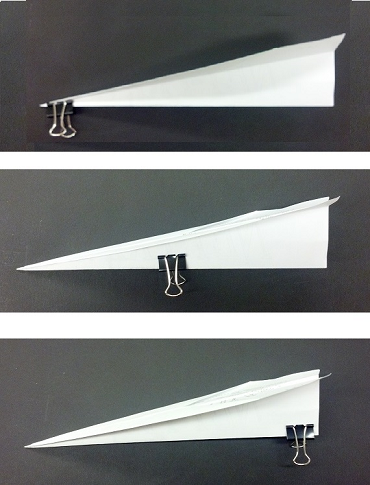
\includegraphics[scale=0.5]{figures/clip.png}
		\caption{We attached a 2.9 gram paper clip to various positions on the paper airplane to shift its center of gravity.}
	\label{fig:clip}
\end{figure}

We then launched the paper airplanes in the manner described in section~\ref{sec:arrow}. To reduce measurement noise, we performed ten launches for each of the paper airplanes at each of the center of gravity settings (a total of 90 launches). To measure flight stability, we recorded the number of x, y, and z-rotations the paper airplane had completed during its flight. See Figure~\ref{fig:rotation} for a classification of these rotations. We also measured the distance traveled when the paper airplane landed. A stable flight should have very few rotations and consistent distance traveled. Figure~\ref{fig:centerofgravity} shows the result. 

\begin{figure}[hl]
	\centering
		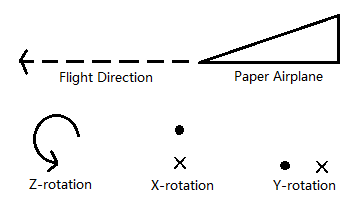
\includegraphics[scale=0.8]{figures/rotation.png}
		\caption{A schematic illustrating different types of rotation during flight.}
	\label{fig:rotation}
\end{figure}

\begin{figure}[hl]
	\centering
		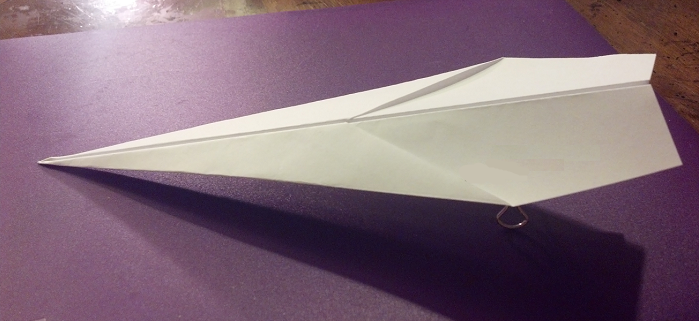
\includegraphics[scale=0.7]{figures/centerofgravity.png}
		\caption{Flight stability vs the center of gravity. Flight distance standard deviation and number of rotations in the air provide qualitative measures of stability: the smaller the standard deviation and fewer the number of rotation, the more stable the flight. We shifted the flight's center of gravity by attaching a metal clip to various positions on the paper airplane.}
	\label{fig:centerofgravity}
\end{figure}

When the clip was attached at the rear of the paper airplane, we observed both y and z-rotations. The flight was extremely turbulent and the paper airplane lost direction soon after launch. As a result, the distance traveled was short. When the clip was attached to the front or the middle of the paper airplane, no rotation was observed during flight. To compare the stability, we looked at the standard deviation of distance. When the clip was attached to the front, the standard deviation was smaller, indicating more consistent and stable flights. In conclusion, we found that the stability of flight decreases as the center of gravity shifts towards the rear of the airplane. This supports our analysis in section~\ref{sec:long_stability}. One interesting thing to notice is that when the clip was attached to the middle of the paper airplane, the distance traveled was the longest. This suggests there's a possible trade-off between stability and lift coefficient. 


\subsection{Stability vs Wing Angles}
As discussed in section~\ref{sec:dehydral}, wing angle has a direct effect on flight stability. To test this, we used Scotch tape to fix the wing at a dihedral(45 degrees above horizon) and an anhidral(45 degrees below horiozn) configuration. We then launched each of the three paper airplanes ten times at both angles, in the manner described in section~\ref{sec:arrow}. We recorded the average distance and number of rotations in air. See Figure~\ref{fig:angles}. 

\begin{figure}[hl]
	\centering
		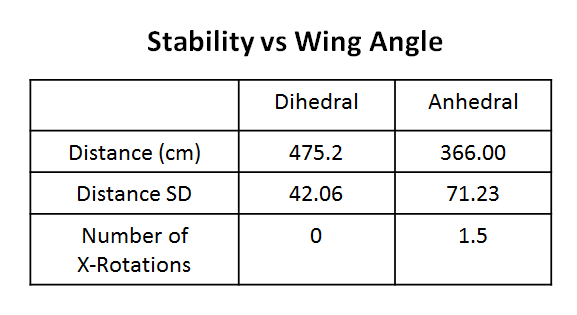
\includegraphics[scale=0.5]{figures/angles.png}
		\caption{Flight distance and stability at different wing angles.}
	\label{fig:angles}
\end{figure}

At dihedral setting, the paper airplanes traveled longer. The flights were also more stable when the wing was dihedral, as shown by the smaller SD and zero number of rotation. 

\subsection{Flight Distance and Stability vs Aspect Ratio}

To explore the relation between flight range/stability and aspect ratio, we constructed four The Arrow models with different aspect ratios. We used paper of
different dimensions but the same area in order to control the paper airplane weight. We then launched each of them in the manner described in section~\ref{sec:arrow}, and recorded the flight distance and stability data. To reduce measurement noise, we tested each paper airplane ten times and used the average value. See Figure~\ref{fig:aspectratioresult} for the result. 


\begin{figure}[hl]
	\centering
		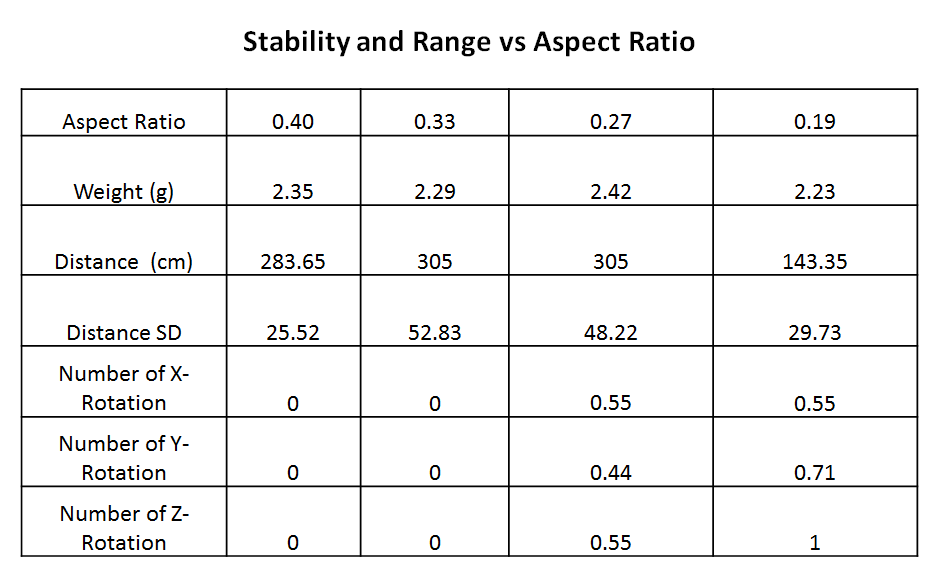
\includegraphics[scale=0.7]{figures/aspectratioresult.png}
		\caption{Flight distance and stability vs aspect ratios.}
	\label{fig:aspectratioresult}
\end{figure}



The result supports the predictions in section XXX. As aspect ratio increases, the flight becomes XXX and XXX. It's worth noticing that when the aspect ratio is larger than XXX, we observed a flapping motion of the wing. The flight became very unstable and the data were ignored.
